%======================================================================
\chapter{Experimental Results}
%======================================================================
\label{ch:exp}

\begin{sidewaystable*}[htbp]
\centering
\caption{Ranking effectiveness on Robust04, Core17 and Core18}
\begin{center}
\resizebox{\columnwidth}{!}{
\begin{tabular}{lcc ccc ccc ccc}
\toprule
 & \multicolumn{3}{c}{\textbf{Robust04}} & \multicolumn{3}{c}{\textbf{Core17}} & \multicolumn{3}{c}{\textbf{Core18}} \\
 \cmidrule(lr){2-4}  \cmidrule(lr){5-7}  \cmidrule(lr){8-10}
{\bf Model} & {\bf MAP} & {\bf P@20} & {\bf NDCG@20}   & {\bf MAP}  & {\bf P@20} & {\bf NDCG@20} & {\bf MAP} & {\bf P@20} & {\bf NDCG@20}  \\
\toprule
BM25+RM3 & 0.2903 & 0.3821 & 0.4407 & 0.2823 & 0.5500 & 0.4467 & 0.3135 & 0.4700 & 0.4604 \\
\midrule
1S: $ \textrm{BERT}(\textrm{MB}) $ & 0.3408$^{\dagger}$ & 0.4335$^{\dagger}$ & 0.4900$^{\dagger}$ & 0.3091$^{\dagger}$ & 0.5620 & 0.4628 & 0.3393$^{\dagger}$ & 0.4930 & 0.4848$^{\dagger}$  \\
2S: $ \textrm{BERT}(\textrm{MB}) $ & 0.3435$^{\dagger}$ & 0.4386$^{\dagger}$ & 0.4964$^{\dagger}$ & 0.3137$^{\dagger}$ & 0.5770 & 0.4781 & 0.3421$^{\dagger}$ & 0.4910 & 0.4857$^{\dagger}$  \\
3S: $ \textrm{BERT}(\textrm{MB}) $ & 0.3434$^{\dagger}$ & 0.4422$^{\dagger}$ & 0.4998$^{\dagger}$ & 0.3154$^{\dagger}$ & 0.5880 & 0.4852$^{\dagger}$ & 0.3419$^{\dagger}$ & 0.4950$^{\dagger}$ & 0.4878$^{\dagger}$ \\
\midrule
1S: $ \textrm{BERT}(\textrm{CAR}) $ & 0.3025$^{\dagger}$ & 0.3970$^{\dagger}$ & 0.4509 & 0.2814$^{\dagger}$ & 0.5500 & 0.4470 & 0.3120 & 0.4680 & 0.4586 \\
2S: $ \textrm{BERT}(\textrm{CAR}) $ & 0.3025$^{\dagger}$ & 0.3970$^{\dagger}$ & 0.4509 & 0.2814$^{\dagger}$ & 0.5500 & 0.4470 & 0.3116 & 0.4670 & 0.4585 \\
3S: $ \textrm{BERT}(\textrm{CAR}) $ & 0.3025$^{\dagger}$ & 0.3970$^{\dagger}$ & 0.4509 &  0.2814$^{\dagger}$ & 0.5500 & 0.4470 & 0.3113 & 0.4670 & 0.4584 \\
\midrule
1S: $ \textrm{BERT}(\textrm{MS MARCO}) $ & 0.3028$^{\dagger}$ & 0.3964$^{\dagger}$ & 0.4512 & 0.2817$^{\dagger}$ & 0.5500 & 0.4468 & 0.3121 & 0.4670 & 0.4594 \\
2S: $ \textrm{BERT}(\textrm{MS MARCO}) $ & 0.3028$^{\dagger}$ & 0.3964$^{\dagger}$ & 0.4512 & 0.2817$^{\dagger}$ & 0.5500 & 0.4468 & 0.3121 & 0.4670 & 0.4594 \\
3S: $ \textrm{BERT}(\textrm{MS MARCO}) $ & 0.3028$^{\dagger}$ & 0.3964$^{\dagger}$ & 0.4512 & 0.2817$^{\dagger}$ & 0.5500 & 0.4468 & 0.3121 & 0.4670 & 0.4594 \\
\midrule
1S: $ \textrm{BERT}(\textrm{CAR}\rightarrow\textrm{MB}) $ & 0.3476$^{\dagger}$ & 0.4380$^{\dagger}$ & 0.4988$^{\dagger}$ & 0.3103$^{\dagger}$ & 0.5830 & 0.4758 & 0.3385$^{\dagger}$ & 0.4860 & 0.4785 \\
2S: $ \textrm{BERT}(\textrm{CAR}\rightarrow\textrm{MB}) $ & 0.3470$^{\dagger}$ & 0.4400$^{\dagger}$ & 0.5015$^{\dagger}$ & 0.3140$^{\dagger}$ & 0.5830 & 0.4817$^{\dagger}$ & 0.3386$^{\dagger}$ & 0.4810 & 0.4755 \\
3S: $ \textrm{BERT}(\textrm{CAR}\rightarrow\textrm{MB}) $ & 0.3466$^{\dagger}$ & 0.4398$^{\dagger}$ & 0.5014$^{\dagger}$ & 0.3143$^{\dagger}$ & 0.5830 & 0.4807 & 0.3382$^{\dagger}$ & 0.4830 & 0.4731 \\
\midrule
1S: $ \textrm{BERT}(\textrm{MS MARCO}\rightarrow\textrm{MB}) $ & 0.3676$^{\dagger}$ & 0.4610$^{\dagger}$ & 0.5239$^{\dagger}$ & 0.3292$^{\dagger}$ & 0.6080$^{\dagger}$ & 0.5061$^{\dagger}$ & 0.3486$^{\dagger}$ & {\bf 0.4920} & {\bf 0.4953}$^{\dagger}$ \\
2S: $ \textrm{BERT}(\textrm{MS MARCO}\rightarrow\textrm{MB}) $ & {\bf 0.3697}$^{\dagger}$ & 0.4657$^{\dagger}$ & 0.5324$^{\dagger}$ & {\bf 0.3323}$^{\dagger}$ & 0.6170$^{\dagger}$ & {\bf 0.5092}$^{\dagger}$ & 0.3496$^{\dagger}$ & 0.4830 & 0.4899$^{\dagger}$ \\
3S: $ \textrm{BERT}(\textrm{MS MARCO}\rightarrow\textrm{MB}) $ & 0.3691$^{\dagger}$ & {\bf 0.4669}$^{\dagger}$ & {\bf 0.5325}$^{\dagger}$ & 0.3314$^{\dagger}$ & {\bf 0.6200}$^{\dagger}$ & 0.5070$^{\dagger}$ & {\bf 0.3522}$^{\dagger}$ & 0.4850 & 0.4899$^{\dagger}$ \\
\bottomrule
\end{tabular}
}
\label{tab:results}
\end{center}
\end{sidewaystable*}

\section{Datasets}

We conduct end-to-end document ranking experiments on three TREC newswire collections:\
the Robust Track from 2004 (Robust04) and the Common Core Tracks from 2017 and 2018 (Core17 and Core18).

\subsubsection{Robust04}

Robust04 draws from the TREC Robust Track in 2004, which is the set of documents from TREC Disks 4 and 5, spanning news articles from Financial Times and LA Times, except the Congressional Record.
The dataset comprises 250 topics, with relevance judgments on a collection of 500K documents.
The goal of the Robust track is to improve the consistency and robustness of retrieval methods by focusing search on poorly performing topics .
Specifically, this task involves searching across a fixed set of documents using previously unseen topics.
Notably the lengths of documents in Robust04 are highly biased:\ \myworries{data}, which is difficult for neural text matching models to handle.
\myworries{What does this mean for us?}

\subsubsection{Core17 \& Core18}

Core17 and Core18 are based on the TREC 2017 and 2018 Common Core Tracks respectively.
The motivation behind these tracks is to build up-to-date test collections based on more recently created documents.
\myworries{that avoids the pitfalls of depth-k pooling}
Core17 uses 1.8M articles from the New York Times Annotated Corpus
while Core18 uses around 600K articles from the TREC Washington Post Corpus.
Core17 and Core18 have only 50 topics each, which are drawn from the Robust Track topics.

\section{Results and Analyses}

Table \ref{tab:results} presents our main results on Robust04, Core17 and Core18.
The top row, BM25+RM3, corresponds to the BM25 runs with RM3 query expansion using default Anserini parameters.
Although higher scores can be obtained on Robust04 with tuned parameters, we present untuned runs for the sake of fairness as no careful tuning has been performed for Core17 or Core18.
The remaining five blocks show the retrieval effectiveness of our models trained as described in Section \myworries{X}.
The models are labeled to reflect the fine-tuning procedure where the datasets that a $ \textrm{BERT}_{\textrm{\scriptsize Large}} $ model was trained on are listed in order in parantheses.
The $ n $S preceding the model name indicates that the top $ n$ sentences were interpolated to compute an overall document score.
Table \ref{tab:results} also highlights statistically significant results based on paired $ t $-tests compared to the BM25+RM3 baseline with $ {\dagger} $.
We report significance at the $ p<0.0 1$ level, with appropriate Bonferroni corrections for multiple hypothesis testing.

\subsection{Effect of Training Data}

By fine-tuning BERT on three different datasets alone and in combination, we hope to study the effect of nature and amount of training data on the power of our learned relevance matching model.
As Table \ref{tab:results} shows, the particular source of relevance labels that we train BERT on \myworries{dramatically} influences retrieval effectiveness across all three collections.

First of all, we find that fine-tuning BERT on MB alone, i.e: $ \textrm{BERT}(\textrm{MB}) $, significantly outperforms the BM25+RM3 baseline for all metrics on Robust04.
We observe significant increases in AP on Core17 and Core18 as well \myworries{and in P@20 and NDCG@20 in some cases}.
These results confirm that relevance models learned from tweets can be successfully transferred to news articles in spite of the considerable differences in domain \myworries{and style}.
This surprising finding may be attributed to the relevance matching power of BERT.
\myworries{Reword}
\myworries{MB portion?}

Unlike MB, fine-tuning on MS MARCO or CAR results in marginal gains over the baseline on Robust04.
Reranking with these models in fact hurts effectiveness on Core17 and Core18 across all metrics.
The synthetic nature of CAR data especially does not appear to be useful for relevance modeling on newswire collections.
For instance, $ \textrm{BERT}(\textrm{CAR}) $ leads to 0.3120 AP on Core18 compared to the 0.3135 AP of the baseline, which means that the model actually picks irrelevant documents as the most relevant to the query.
As the results $ 2S $ and $ 3S $ for the same model show, the effectiveness on Core18 in fact progressively degrades the more sentences are considered in final score aggregation.
Intuitively these results indicate that using these models disrupt the order imposed by the baseline.
For the other experiments with these two models. the number of sentences considered does not seem to affect effectiveness at all.

Results with $ \textrm{BERT}(\textrm{MS MARCO}) $ are more surprising in that the MS MARCO dataset captures a search task, and web passages in the dataset are closer to the newswire test collections than MB in terms of domain.
Given the proximity of domains, it would be reasonable to expect relevance transfer between MS MARCO and newswire collections to be more effective.
However, our results indicate that this is not necessarily the case, and fine-tuning on MS MARCO alone rather than MB alone is far less effective for relevance transfer.

Although fine-tuning on CAR or MS MARCO alone does not yield large improvements, we actually obtain considerably higher results by fine-tuning these models further on MB.
With $ \textrm{BERT}(\textrm{CAR}\rightarrow\textrm{MB}) $ we achieve effectiveness that is slightly better than fine-tuning on MB alone in some cases.
We hypothesize that CAR might have a similar effect to language pre-training in that it doesn't directly apply to the downstream document retrieval task, but provides a better representation that can benefit from fine-tuning on MB.
More surprisingly, fine-tuning on MS MARCO first and then on MB represents our best model ($ \textrm{BERT}(\textrm{MS MARCO}\rightarrow\textrm{MB}) $) as shown in the final block of the table.
This model is able to exploit data from both MS MARCO and MB, with a score that is higher than fine-tuning on each dataset alone.

\subsection{Comparison to Other Ranking Models}

\myworries{Focus on ML-based models}
In this section we try to put our results into perspective by considering them in the larger context of document retrieval research.
For Robust04, we report the highest AP score that we are aware of, 0.3697, with our best model $ \textrm{BERT}(\textrm{MS MARCO}\rightarrow\textrm{MB}) $.
The most effective neural model on Robust04 was reported to be \myworries{X}~\cite{} at 0.3124 AP according to the meta-analysis of over 100 papers up until 2019 on this dataset by \cite{}\footnote{\url{https://github.com/lintool/robust04-analysis}}.
Furthermore, our results with the same model on Robust04 exceed the previous highest known score of 0.3686, which is a non-neural method based on ensembles~\cite{Cormack:2009:RRF:1571941.1572114}.
\myworries{This high water mark has stood unchallenged for ten years.}

More recently, \cite{MacAvaney_etal_SIGIR2019} reported 0.5381 NDCG@20 on Robust04 by integrating contextualized word representations into existing neural ranking models; unfortunately, they did not report AP results.
Our best NDCG@20 on \mbox{Robust04} (0.5325) approaches their results even though we optimize for AP.
Finally, note that since we are only using Robust04 data for learning the document and sentence weights in Eq~(\ref{eq:1}), and not for fine-tuning BERT itself, it is less likely that we are overfitting.

Our best model also achieves a higher AP on Core17 than the best TREC submission that does not make use of past labels or human intervention (\texttt{umass\_baselnrm}, 0.275 AP)~\cite{core2017trec}.
Under similar conditions, we beat every TREC submission in Core18 as well (with the best run being \texttt{uwmrg}, 0.276 AP)~\cite{core2018trec}.
Core17 and Core18 are relatively new and thus have yet to receive much attention from researchers, but to our knowledge, these figures represent the state of the art.

\subsection{Number of Sentences}

In general, we consider up to three top scoring sentences in each document to compute an overall document score.
Our results in Table \ref{tab:results} suggest that the top scoring sentence alone is often a good indicator of document relevance; in fact we achieve the best MAP in about half of the experiments by only considering the most relevant sentence.
This finding is consistent with those of \cite{zhang2018effective} who verified through user studies that the most relevant sentence or paragraph in a document provides a reliable proxy for document relevance.

Considering the next most relevant sentence in addition to the top sentence yields a noticeable increase across all metrics in some of the experiments.
\myworries{This is especially true in the case of better performing models such as $ \textrm{BERT}(\textrm{MS MARCO}\rightarrow\textrm{MB}) $ which might be explained by their ability to effectively match multiple useful sentences.}
However, we find that adding a third in fact causes effectiveness to drop in some cases.
\myworries{Try for more than 3 for a few and compare}
\myworries{Comment for all three metrics and datastes}
\myworries{Conclusion?}

\subsection{Per-Query Error Analysis}

Our results in Table \ref{tab:results} give a good overview of the effect of training data on cross-domain relevance transfer.
However, they do not reveal much concerning the particular strengths and weaknesses of each model compared to the baseline.
To gain further insight into the characteristics of our models, we analyze the per-query retrieval effectiveness of each model compared to the baseline on Robust04, Core17 and Core18.
Figure \myworries{X} plots $\Delta$ AP per query (i.e: $ \texttt{AP}_{\texttt{Model}} - \texttt{AP}_{\texttt{BM25+RM3}} $, sorted in descending order.

\begin{figure}
	\centering
    \begin{minipage}{0.45\textwidth}
        \centering
        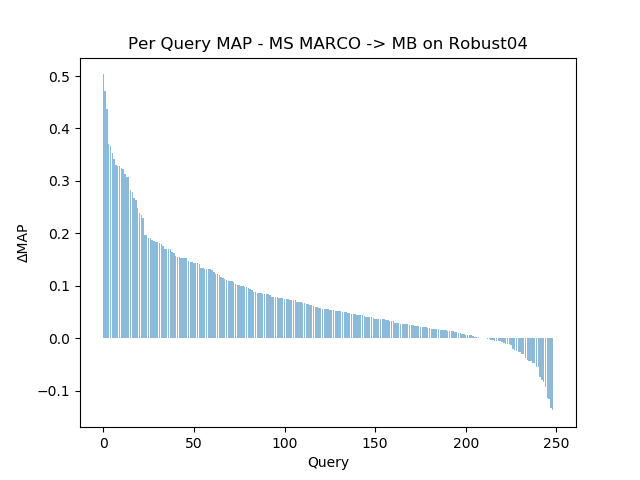
\includegraphics[width=0.9\textwidth]{perquery1.png} % first figure itself
        \caption{first figure}
    \end{minipage}\hfill
    \begin{minipage}{0.45\textwidth}
        \centering
        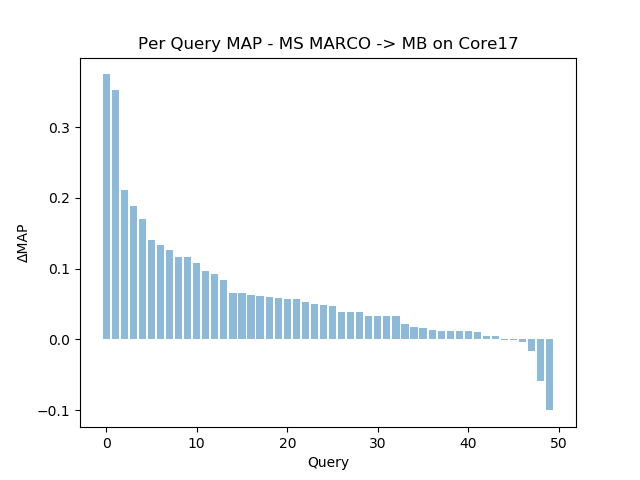
\includegraphics[width=0.9\textwidth]{perquery2.png} % second figure itself
        \caption{second figure}
    \end{minipage}\hfill
    \begin{minipage}{0.45\textwidth}
        \centering
        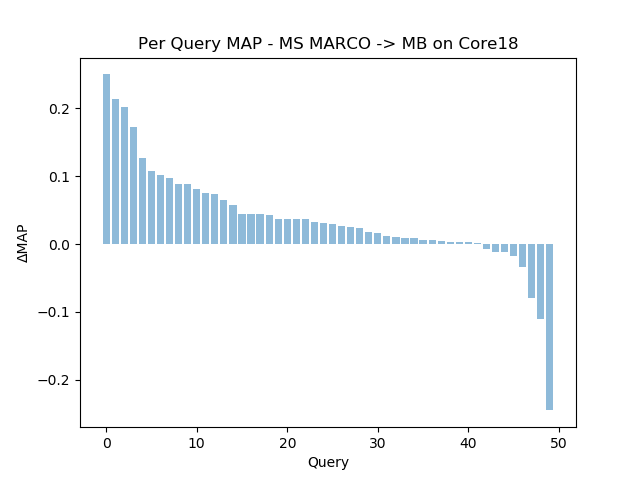
\includegraphics[width=0.9\textwidth]{perquery3.png} % second figure itself
        \caption{second figure}
    \end{minipage}
\end{figure}

\myworries{TODO}

Figure \ref{fig:per_query1}, \ref{fig:per_query2} and \ref{fig:per_query3} show the per query MAP difference between our best model and the baseline.
Our best BERT-based model performs better than the baseline for 83\% of the queries on Robust04, 88\% on Core17 and 84\% on Core18.
This again confirms that BERT is able to capture relevance signals from MS MARCO and MB which directly help with retrieval on our test collecetions.
The best performing queries on Robust04 are \texttt{stirling engine}, \texttt{human stampede} and \texttt{native american casino}, respectively.
The worst performing queries are \texttt{flavr savr tomato}, \texttt{polygamy polyandry polygyny} and \texttt{adult immigrants English}.

\begin{figure}
	\centering
    \begin{minipage}{0.45\textwidth}
        \centering
        \includegraphics[width=0.9\textwidth]{perquery4.png} % first figure itself
        \caption{first figure}
    \end{minipage}\hfill
    \begin{minipage}{0.45\textwidth}
        \centering
        \includegraphics[width=0.9\textwidth]{perquery5.png} % second figure itself
        \caption{second figure}
    \end{minipage}\hfill
    \begin{minipage}{0.45\textwidth}
        \centering
        \includegraphics[width=0.9\textwidth]{perquery6.png} % second figure itself
        \caption{second figure}
    \end{minipage}
\end{figure}

We repeat the same process for our worst model $ \textrm{BERT}(\textrm{CAR}) $ for which we present results in Figures \ref{fig:per_query5}, \ref{fig:per_query5} and \ref{fig:per_query6}.
This model outperforms the baseline only for 57\% of the Robust04 and 34\% of Core18 queries.
%80\% of Core17
It performs especially bad for the query 316 \texttt{polygamy polyandry polygyny} on Robust04 and 802 \texttt{women driving in Saudi Arabia} on Core18.

Overall the query 316 \texttt{polygamy polyandry polygyny} appears to be difficult for BERT based models to correctly judge.
\myworries{Different one?}
In order to compare the characteristics of the two models that cause them to either excel or fail, we look into the ranking of documents for the best and worst performing queries for both.
Specifically, we sample sentences from relevant and non-relevant documents for the given query and compare how their rank these documents.
\myworries{Details!}

% Please add the following required packages to your document preamble:
% \usepackage{multirow}
\begin{table}[]
\begin{tabular}{|c|c|c|c|c|c|}
\hline
\multirow{2}{*}{\textbf{Query}}                       & \multirow{2}{*}{\textbf{Document ID}} & \multirow{2}{*}{\textbf{Sentence}}                                                                                                                                                                                            & \multicolumn{3}{c|}{\textbf{Rank}}                                             \\ \cline{4-6} 
                                                      &                                       &                                                                                                                                                                                                                               & \textbf{Baseline} & \textbf{MS MARCO + MB} & \multicolumn{1}{l|}{\textbf{CAR}} \\ \hline
\multirow{2}{*}{\textbf{372: native american casino}} & LA061290-0112                         & The Sycuan Reservation, one of 18 American Indian reservations in Southern California, operates a gaming center offering high-stakes bingo and poker seven days a week, bringing in more than \$20 million in revenues a year & 223               & 9                      & 197                               \\ \cline{2-6} 
                                                      & FT941-13912                           & Yet, gambling on its own is not enough as Atlantic City, on the east coast in New Jersey, has discovered - to its cost.                                                                                                       & 12                & 38                     & 9                                 \\ \hline
\end{tabular}
\end{table}

\subsection{Effect of Length}

\subsubsection{Query Length}

\begin{table*}[b!]
\centering{
%\begin{tabular}{lll lllll}
\begin{tabular}{lll lllll}
\toprule
 & \multicolumn{5}{c}{\textbf{Query Length}} \\
 \cmidrule(lr){2-6}
{\bf Model} & {\bf 1} & {\bf 2} & {\bf 3}   & {\bf 4}  & {\bf 5} \\
\toprule
BM25+RM3 & 0.3889 & 0.2975 & 0.2760 & 0.3089 & 0.2972 \\
\midrule
$ \textrm{BERT}(\textrm{MB}) $ & 0.4145 & 0.3624 & 0.3229 & 0.3681 & 0.4165 \\
\midrule
$ \textrm{BERT}(\textrm{CAR}) $ & 0.3978 & 0.3112 & 0.2871 & 0.3288 & 0.2844 \\
\midrule
$ \textrm{BERT}(\textrm{MS MARCO}) $ & 0.3997 & 0.3117 & 0.2872 & 0.3289 & 0.2871 \\
\midrule
$ \textrm{BERT}(\textrm{CAR}\rightarrow\textrm{MB}) $ & 0.4202 & 0.3599 & 0.3296 & 0.3757 & 0.4926  \\
\midrule
$ \textrm{BERT}(\textrm{MS MARCO}\rightarrow\textrm{MB}) $ & 0.4253 & 0.3880 & 0.3480 & 0.4077 & 0.5469 \\
\bottomrule
\end{tabular}
}
\caption{\myworries{TODO}}
\label{tab:results-query-length}
\end{table*}

To investigate the ability of our BERT-based models to exploit context-aware representations of the queries, we study the MAP across increasing query lengths.
We conjecture that longer queries would give our models richer context to work with, therefore increasing retrieval effectiveness.
To this end, we categorize the 250 queries from the Robust Track by the number of tokens, and evaluate average MAP per each query length, i.e: from 1 to 5.
This approach is somewhat limited by the narrow range of query lengths, but still gives insight into the effect of query length on each model's \myworries{performance}.

The results for this experiment are shown in Table \ref{tab:results-query-length}.
As expected, the AP for the BM25+RM3 baseline drops by 24\% from a single token query to a query with five tokens.
Other than that, the models produce improvements over the baseline to similar degrees as when they are evaluated over all queries with $ \textrm{BERT}(\textrm{MS MARCO}\rightarrow\textrm{MB}) $ as the best model across all query lengths.
Similar to the baseline, $ \textrm{BERT}(\textrm{CAR}) $ and $ \textrm{BERT}(\textrm{MS MARCO}) $ experience a gradual decline in AP as the query length increases from 1 to 5, leading to an overall 29\% and 28\% decrease respectively.
Note, however, that the decrease in AP is not continuous at each step but reaches a minimum at query length 3 and a maximum at query length 4.
It might be helpful to manually inspect rankings for each query length or to use a different averaging technique less sensitive to sample size in order to better reason about this observation; \myworries{however, we leave this for future work...}
More interestingly, while increasing query length results in a decrease in AP across all the other models, $ \textrm{BERT}(\textrm{MB}) $, $ \textrm{BERT}(\textrm{CAR}\rightarrow\textrm{MB}) $ and $ \textrm{BERT}(\textrm{MS MARCO}\rightarrow\textrm{MB}) $ in fact perform much better at query length 5 than at 1.
Moreover, the performance of the best model  $ \textrm{BERT}(\textrm{MS MARCO}\rightarrow\textrm{MB}) $ degrades much less where the minimum usually occurs, i.e: query length 3, compared to the baseline, $ \textrm{BERT}(\textrm{CAR}) $ and $ \textrm{BERT}(\textrm{MS MARCO}) $.
\myworries{What else?}

\subsubsection{Document Length}

\begin{table*}[t!]
\centering{
\begin{tabular}{lll lll}
\toprule
 & \multicolumn{3}{c}{\textbf{Robust04}} \\
\toprule
BM25+RM3 & 0.2903 & 0.3821 & 0.4407 \\
\midrule
1S: $ \textrm{BERT}_{\textrm{\scriptsize Large}}(\textrm{CAR'}) $ & 0.3030$^{\dagger}$ & 0.3980$^{\dagger}$ & 0.4520 \\
\midrule
1S: $ \textrm{BERT}_{\textrm{\scriptsize Large}}(\textrm{MS MARCO'}) $ & 0.3300$^{\dagger}$ & 0.4309$^{\dagger}$ & 0.4906$^{\dagger}$ \\
\bottomrule
\end{tabular}
}
\caption{Ranking effectiveness on chopped MS MARCO and CAR}
\label{tab:results-chopped}
\end{table*}

It is interesting to note that fine-tuning on MS MARCO or CAR alone results in marginal improvements over the baseline.
Considering any number of top scoring sentences, $ \textrm{BERT}(\textrm{CAR}) $ and $ \textrm{BERT}(\textrm{MS MARCO}) $ both have around 1.2 AP higher than BM25+RM3 on Robust04 with similar gains in P@20 and NDCG@20.
Although still statistically significant, these improvements are much lower than those gained with fine-tuning on MB (5 AP).

We attribute this phenomenon to the length mismatch between the training and evaluation text lengths.
After dividing into chunks that fit the input span that BERT can handle, the average sentence length in Robust04, Core17 and Core18 sentences is 19 tokens long, which is similar to the average number of tokens in MB training at 15.
However, both MS MARCO and CAR \myworries{give statistics}

To validate this hypothesis, we try dividing MS MARCO and CAR passages into chunks the same size as Robust04 sentences.
We find that retrieval effectiveness slightly improves upon fine-tuning on the shortened datasets although much less so than expected.
From this finding we infer that while comparable document length is an important consideration for cross-domain relevance transfer, there may be other factors at play in terms of \myworries{X}.
\myworries{Future work...}

\subsection{Matching Tendencies}

\subsubsection{Semantic Matching}

\begin{table*}[b!]
\centering{
\begin{tabular}{lll lll}
\toprule
 & \multicolumn{3}{c}{\textbf{Pruned Robust04}} \\
 \cmidrule(lr){2-4}
{\bf Model} & {\bf AP} & {\bf P@20} & {\bf NDCG@20}  \\
\toprule
BM25+RM3 & 0.2903 & 0.3821 & 0.4407 \\
\midrule
$ \textrm{BERT} (\textrm{MB}) $ & 0.3031 & 0.4014 & 0.4580 \\
\midrule
$ \textrm{BERT} (\textrm{CAR}) $ & 0.2959 & 0.3936 & 0.4480 \\
\midrule
$ \textrm{BERT} (\textrm{MS MARCO}) $ & 0.2962 & 0.3936 & 0.4483 \\
\midrule
$ \textrm{BERT} (\textrm{CAR}\rightarrow\textrm{MB}) $ & 0.3037 & 0.3998 & 0.4527 \\
\midrule
$ \textrm{BERT} (\textrm{MS MARCO}\rightarrow\textrm{MB}) $ & 0.3101 & 0.4102 & 0.4639 \\
\bottomrule
\end{tabular}
}
\caption{\myworries{TODO}}
\label{tab:results-pruned}
\end{table*}

To isolate the contribution of BERT, we filter sentences in Robust04 that don't contain any of the query terms.
This essentially eliminates the impact of exact matching on the sentence relevance scores, allowing us to verify whether our BERT-based models successfully leverage semantic matching.
Table \ref{tab:results-pruned} displays the retrieval effectiveness of all models on the ``pruned'' Robust04.
Filtering Robust04 sentences leads to a decrease in all metrics across all models, which indicates that exact matching signals are still valuable in relevance predictions.
However, notice that the \myworries{performance} of all models still beats the baseline, which implies that they indeed perform semantic matching with notable gains.
The improvements over the baseline follow the same trend as the results in Table \ref{tab:results}.
While $ \textrm{BERT} (\textrm{CAR}) $ and $ \textrm{BERT} (\textrm{MS MARCO}) $ yield minor improvements over the baseline, the best performing model $ \textrm{BERT} (\textrm{MS MARCO}\rightarrow\textrm{MB}) $ is \myworries{significantly} higher.
\myworries{Significance testing}
Interestingly, the drop in AP caused by filtering sentences is also the highest for the best performing model, indicating that this model is able to exploit both exact and semantic matching signals.
The overall effectiveness of this model on the original Robust04 dataset shown in Table \ref{tab:results} may be owing to the joint matching power demonstrated in this experiment.

\subsubsection{Query Terms}

\begin{table*}[t!]
\centering{
\begin{tabular}{lll lllll}
\toprule
 & \multicolumn{5}{c}{\textbf{Fraction of Query Term}} \\
 \cmidrule(lr){2-6}
{\bf Model} & {\bf [0.0, 0.01)} & {\bf [0.01, 0.02)} & {\bf [0.02, 0.03)} \\
\toprule
BM25+RM3 &  \\
\midrule
$ \textrm{BERT}(\textrm{MB}) $ &  \\
\midrule
$ \textrm{BERT}(\textrm{CAR}) $ &  \\
\midrule
$ \textrm{BERT}(\textrm{MS MARCO}) $ &  \\
\midrule
$ \textrm{BERT}(\textrm{CAR}\rightarrow\textrm{MB}) $ &   \\
\midrule
$ \textrm{BERT}(\textrm{MS MARCO}\rightarrow\textrm{MB}) $ &  \\
\bottomrule
\end{tabular}
}
\caption{\myworries{TODO}}
\label{tab:results-query-terms}
\end{table*}

BM25 favors documents with frequent occurrences of query terms which is not necessarily the case of our BERT-based models.
\myworries{Hypothesis}
Therefore, we calculate the fraction of query terms (FQT) in the top k documents for each query across all models, removing stopwords and punctuation.
We average the FQT across all retrieved documents for each query:

\begin{equation}
FQT(q) = \frac{1}{k} \sum^k _{i=1} \frac{N(d_i, q)}{|d_i|}
\end{equation}

where $ N(d_i, q) $ denotes the number of occurrences fo query tokens $ q $ in document $ d_i $.
\myworries{limit k to 10 to avoid noise?}
\myworries{Divide into 3 buckets instead?}
\myworries{FQT average for each model}
\myworries{Comment}

Because BM25 relies too much on query term frequency, it may rank documents that contain multiple repetitions of query words but do not actually convey any useful information too highly.
Therefore, we expect the effectiveness of BM25 to drop more significantly with increasing FQT.
To observe how retrieval effectiveness changes across different ranges of FQT, we split the values into \myworries{X} buckets and calculate the average MAP for each bucket.
\myworries{Comment}
\myworries{Give examples of useless high FQT}

\subsection{Novel Terms}

Pretrained on massive amounts of data for language modeling, BERT can capture various semantic relationships helpful for relevance prediction.
Figures \myworries{X} one of the top scoring sentences for the query 322 \texttt{international art crime}.
Note that the sentence does not contain any exact matches with the query terms and is nonetheless relevant to the query.

\myworries{description}
\myworries{This highlights the power of...}

\myworries{MS MARCO MB}
\begin{figure}
	\centering
    \begin{minipage}{0.45\textwidth}
        \centering
        \includegraphics[width=0.9\textwidth]{vis1.png} % first figure itself
        \caption{first figure}
    \end{minipage}\hfill
    \begin{minipage}{0.45\textwidth}
        \centering
        \includegraphics[width=0.9\textwidth]{vis2.png} % second figure itself
        \caption{second figure}
    \end{minipage}\hfill
    \begin{minipage}{0.45\textwidth}
        \centering
        \includegraphics[width=0.9\textwidth]{vis3.png} % second figure itself
        \caption{second figure}
    \end{minipage}
\end{figure}

\begin{figure}
	\centering
    \begin{minipage}{0.45\textwidth}
        \centering
        \includegraphics[width=0.9\textwidth]{vis4.png} % first figure itself
        \caption{first figure}
    \end{minipage}\hfill
    \begin{minipage}{0.45\textwidth}
        \centering
        \includegraphics[width=0.9\textwidth]{vis5.png} % second figure itself
        \caption{second figure}
    \end{minipage}\hfill
    \begin{minipage}{0.45\textwidth}
        \centering
        \includegraphics[width=0.9\textwidth]{vis6.png} % second figure itself
        \caption{second figure}
    \end{minipage}
\end{figure}